\section{Evaluation}\label{chapter.discussion}
\thispagestyle{plain}

This chapter opens with introducing a collection of test sets used to measure the performance of the allocations mechanism OptiX through experiments, and compare it to the performance of ORX on the same collection. The results are evaluated and discussed, followed by an assessment of factors that may threat the validity of the results obtained in the experimental phase. \toolname \space is then discussed and evaluated as a whole, before the chapter rounds off by discussing the return on the investment put into this project.

\comment{
\subsection{Research Questions?}
Look at Mortens report for inspiration. Or maybe not?
}

\subsection{Experimental Evaluation of Test Allocation}
%\improvement[inline]{TODO}
\comment{- Present test data, run experimental tests and create tables and charts, include a second version of ORX that runs without interruption in order to compare OptiX and ORX to the actual optimal overall running duration!}

In order to measure and evaluate the performance of OptiX, which represented a major objective in this project, an experimental evaluation was performed on OptiX as well as on ORX to establish benchmark values.

The test data used in the experimental evaluation is divided into four collections, each consisting of three pseudo test sets. The test sets in each collection all represent scenarios with a given number of tests and available machines. What separates the test sets in the same collection is the number of machines each test in the test set can be executed on. Each collection contains one test set in which every test can be executed on every machine, one where the tests can only be executed on a small selection of the machines 

\begin{landscape}
    \thispagestyle{plain}
    \vspace*{\fill}
    \begin{table}[h]
      \begin{tabular}{|c|c|c|c|c|}
        \hline
        \textbf{Collection} & \textbf{Tests} & \textbf{Machines} & \textbf{Test Set} & \textbf{No. of Machines Tests are Executable On}\\
        \hline
        \multirow{3}{*}{$c_1$} & \multirow{3}{*}{1000} & \multirow{3}{*}{100} & $ts_{1}$  & 100\\
                               &                       &                      & $ts_{2}$  & 10\\
                               &                       &                      & $ts_{3}$  & \emph{Random}\\
        \hline
        \multirow{3}{*}{$c_2$} & \multirow{3}{*}{1000} & \multirow{3}{*}{10}  & $ts_{4}$  & 10\\
                               &                       &                      & $ts_{5}$  & 5\\
                               &                       &                      & $ts_{6}$  & \emph{Random}\\
        \hline
        \multirow{3}{*}{$c_3$} & \multirow{3}{*}{200} & \multirow{3}{*}{50}   & $ts_{7}$  & 50\\
                               &                      &                       & $ts_{8}$  & 10\\
                               &                      &                       & $ts_{9}$  & \emph{Random}\\
        \hline
        \multirow{3}{*}{$c_4$} & \multirow{3}{*}{200} & \multirow{3}{*}{10}   & $ts_{10}$ & 10\\
                               &                      &                       & $ts_{11}$ & 5\\
                               &                      &                       & $ts_{12}$ & \emph{Random}\\
        \hline
      \end{tabular}
      \centering
      \caption{Test Data}
      \label{test_data}
    \end{table}
    \vspace*{\fill}
\end{landscape}

\noindent and one where the number of machines each test can be executed on varies and is determined at random. This means that there is also a varying number of combinatorial solutions to the optimization problem.

Table \ref{test_data} shows details about the test data which is randomly generated; only the number of tests, test machines and how many machines each test is executable on was specified upon generation. Each test was assigned a duration between 30 and 120 seconds, and a set of machines on which they were executable on, both generated at random. The test data is designed to imitate realistic scenarios, although somewhat amplified. Using larger test sets than $ts_1$ through $ts_3$ would not be very meaningful, as 1000 tests and 100 test machines are very large numbers in this context, and are not likely to be exceeded any time soon.

The test sets, located in \emph{/controller/test\_data/input/}, are stored as JSON objects in files with the naming convention \emph{{test\_set\_x.json}}, where \emph{x} represents the number of the test set. Likewise, the results from the experimental testing are stored in files with the same naming convention, but in \emph{/controller/test\_data/output/} instead.

\begin{table}[h]
    \centering
  \footnotesize
  \begin{tabular}{|c|ccc|ccc|}
    \hline
    &  \multicolumn{3}{c|}{\textbf{\large{OptiX}}} & \multicolumn{3}{c|}{\textbf{\large{ORX}}}\\
    \emph{Test Set} & \emph{$T_s$} & \emph{$T_e$} & \emph{$T_t$} & \emph{$T_s$} & \emph{$T_e$} & \emph{$T_t$}\\
    \hline
    $ts_{1}$   &   $30.04s$    &   $777.00s$     &   $\mathbf{807.04s}$     &   $34.93s$    &   $1153.00s$   &   $\mathbf{1187.93s}$ \\
    $ts_{2}$   &   $8.66s$     &   $752.00s$     &   $\mathbf{760.66s}$     &   $34.25s$    &   $1224.00s$   &   $\mathbf{1258.25s}$ \\
    $ts_{3}$   &   $0.29s$     &   $867.00s$     &   $\mathbf{867.29s}$     &   $34.44s$    &   $1172.00s$   &   $\mathbf{1206.44s}$ \\
    \hline
    $ts_{4}$   &   $0.02s$     &   $7410.00s$    &   $\mathbf{7410.02s}$    &   $30.37s$    &   $7797.00s$   &   $\mathbf{7827.37s}$ \\
    $ts_{5}$   &   $0.16s$     &   $7497.00s$    &   $\mathbf{7497.16s}$    &   $30.27s$    &   $7569.00s$   &   $\mathbf{7599.27s}$ \\
    $ts_{6}$   &   $0.19s$     &   $7354.00s$    &   $\mathbf{7354.19s}$    &   $30.26s$    &   $7773.00s$   &   $\mathbf{7803.26s}$ \\
    \hline
    $ts_{7}$   &   $1.72s$     &   $301.00s$     &   $\mathbf{302.72s}$     &   $30.39s$    &   $365.00s$    &   $\mathbf{395.39s}$  \\
    $ts_{8}$   &   $0.22s$     &   $355.00s$     &   $\mathbf{355.22s}$     &   $30.27s$    &   $338.00s$    &   $\mathbf{368.27s}$  \\
    $ts_{9}$   &   $0.67s$     &   $311.00s$     &   $\mathbf{311.67s}$     &   $30.36s$    &   $319.00s$    &   $\mathbf{349.36s}$  \\
    \hline
    $ts_{10}$  &   $0.18s$     &   $1428.00s$    &   $\mathbf{1428.18s}$    &   $30.06s$    &   $1435.00s$   &   $\mathbf{1465.06s}$ \\
    $ts_{11}$  &   $0.60s$     &   $1520.00s$    &   $\mathbf{1520.60s}$    &   $30.06s$    &   $1553.00s$   &   $\mathbf{1583.06s}$ \\
    $ts_{12}$  &   $0.80s$     &   $1549.00s$    &   $\mathbf{1549.80s}$    &   $30.06s$    &   $1531.00s$   &   $\mathbf{1561.06s}$\\
    \hline
  \end{tabular}
  \caption{Experimental Test Results}
  \label{test_results}
\end{table}

Both OptiX and ORX were tested with each of these 12 pseudo test sets. The results can be found in Table \ref{test_results}, which provides searching time, execution time and total time obtained with both allocation mechanisms for each test set. As explained in the formal definition of the optimization problem in Chapter \ref{chapter.background}, the objective of the problem was to minimize the $T_{t} = T_{e} + T_{s}$, that is to say the searching time used to find the solution plus the execution time used to execute the tests.

\begin{landscape}
    \begin{figure}[p]
        \centering
        \thisfloatpagestyle{plain}
        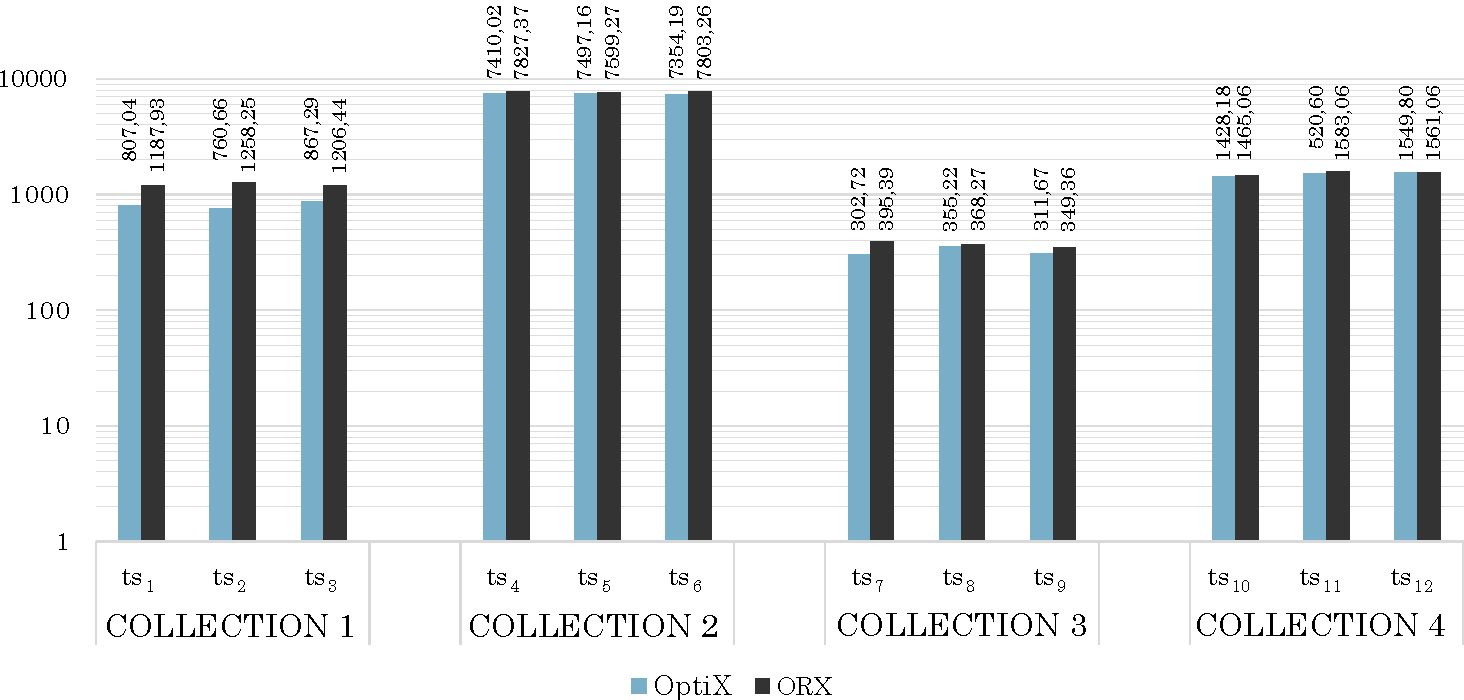
\includegraphics[scale=0.82]{figures/test_results/all.pdf}
        \caption{Complete Results from Experimental Evaluation}
        \label{fig.expres}
    \end{figure}
\end{landscape}

The complete results from the experimental evaluation are visualized in Figure \ref{fig.expres}. Because of major variations in numbers, a logarithmic scale is used in the graph. The results from each collection will subsequently be discussed individually.

\begin{figure}[t]
    \centering
    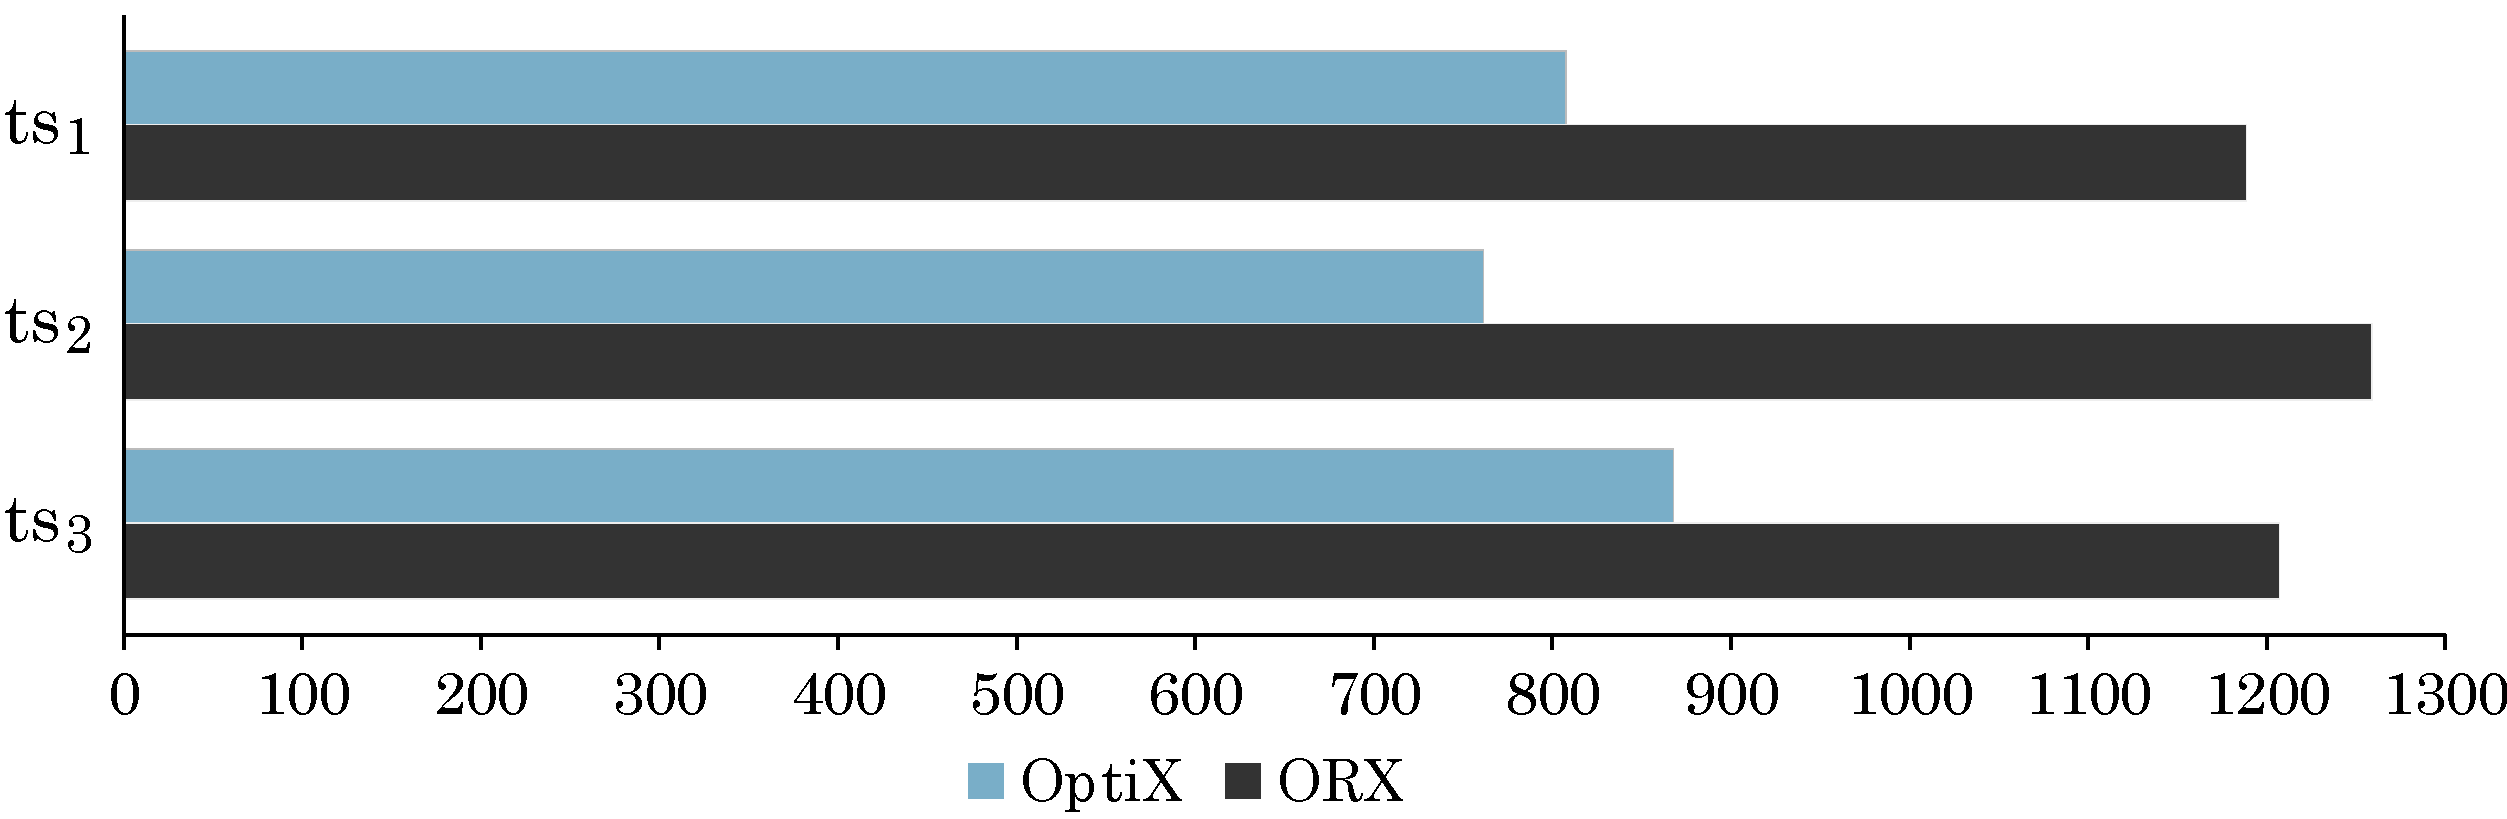
\includegraphics[width=\textwidth]{figures/test_results/1.pdf}
    \caption{Results from Test Data Collection 1 in Experimental Evaluation}
    \label{1st_test_set}
\end{figure}

The first collection of test sets consisted of $ts_1$, $ts_2$ and $ts_3$, with 1000 tests and 100 test machines. This collection was designed to test the mechanisms in situations with a large number of both tests and machines, and an abundance of possible solutions.

As we can see from Figure \ref{1st_test_set}, OptiX provided excellent results compared to ORX for these test sets. Not only were all of the execution times provided by OptiX between 305 and 472 seconds faster than ORX; it also provided better searching times. $ts_1$ was the test set with the most possible solutions, as all tests could be executed on all machines, and thus the only test set with which OptiX timed out after 30 seconds. Although the searching process of ORX timed out after 30 seconds, the whole process took just over 34 seconds in all of these cases, which can likely be explained by the post-processing time being extended as a consequence of large numbers of tests and machines. This was the collection in which the results provided by OptiX was the most prominent.

\begin{figure}[t]
    \centering
    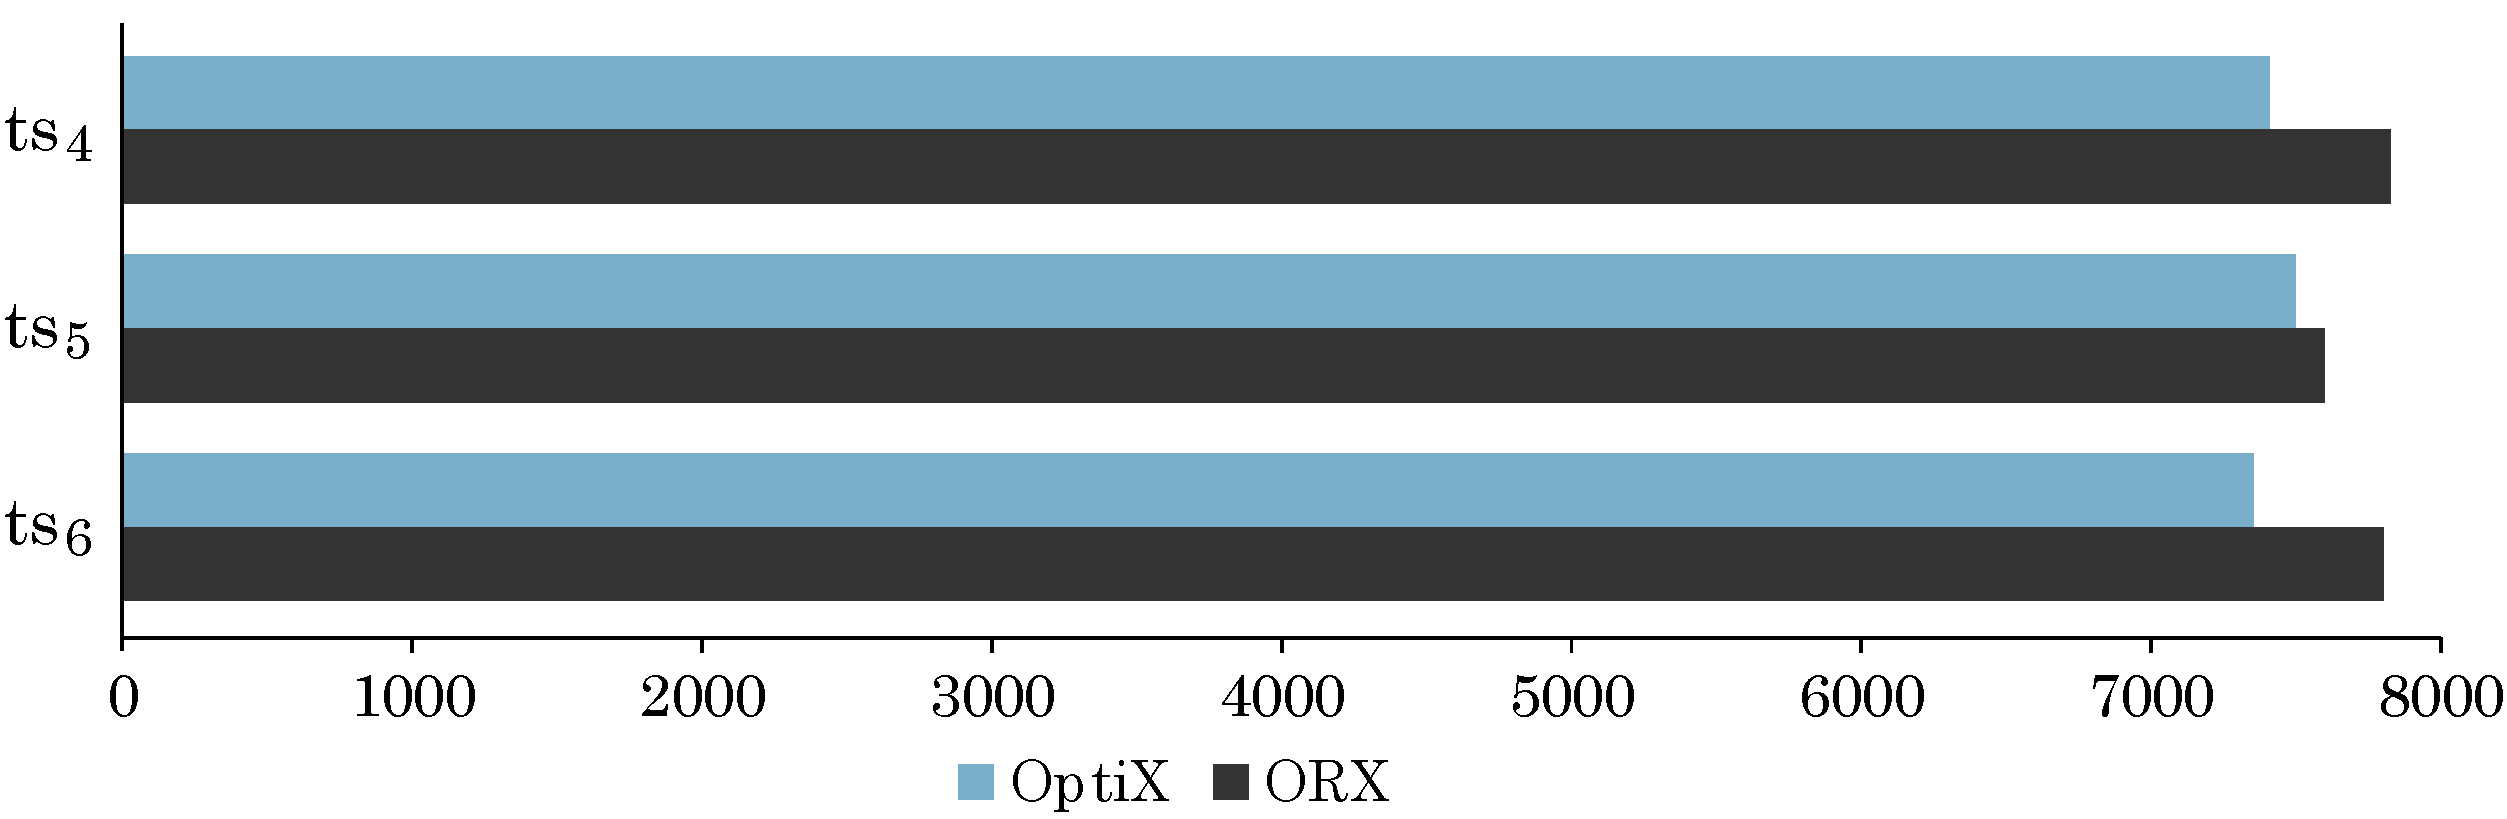
\includegraphics[width=\textwidth]{figures/test_results/2.pdf}
    \caption{Results from Test Data Collection 2 in Experimental Evaluation}
    \label{2nd_test_set}
\end{figure}

The second collection of test sets consisted of $ts_4$, $ts_5$ and $ts_6$, with 1000 tests and 10 test machines, and was designed to test the mechanisms in situations with a large number of tests and a small number of machines.

Figure \ref{2nd_test_set} shows that even though OptiX provided better total time than ORX on all test sets, the difference between the two mechanisms is less prominent in this collection than in the previous one. The largest difference in total time is 449.07 seconds for $ts_6$, and the smallest 102.11 seconds for $ts_5$, which are both small numbers considering that the total duration is more than two hours for both mechanisms on each test set. The  is likely linked to the much smaller number of possible solutions in the test sets in this collection compared to the first one. Nevertheless, OptiX undeniably outperformed ORX in searching time, where OptiX used less than a second on each test set and ORX timed out after 30 seconds, as well as in the execution time, and thus the total time on all test sets in this collection.

\begin{figure}[b]
    \centering
    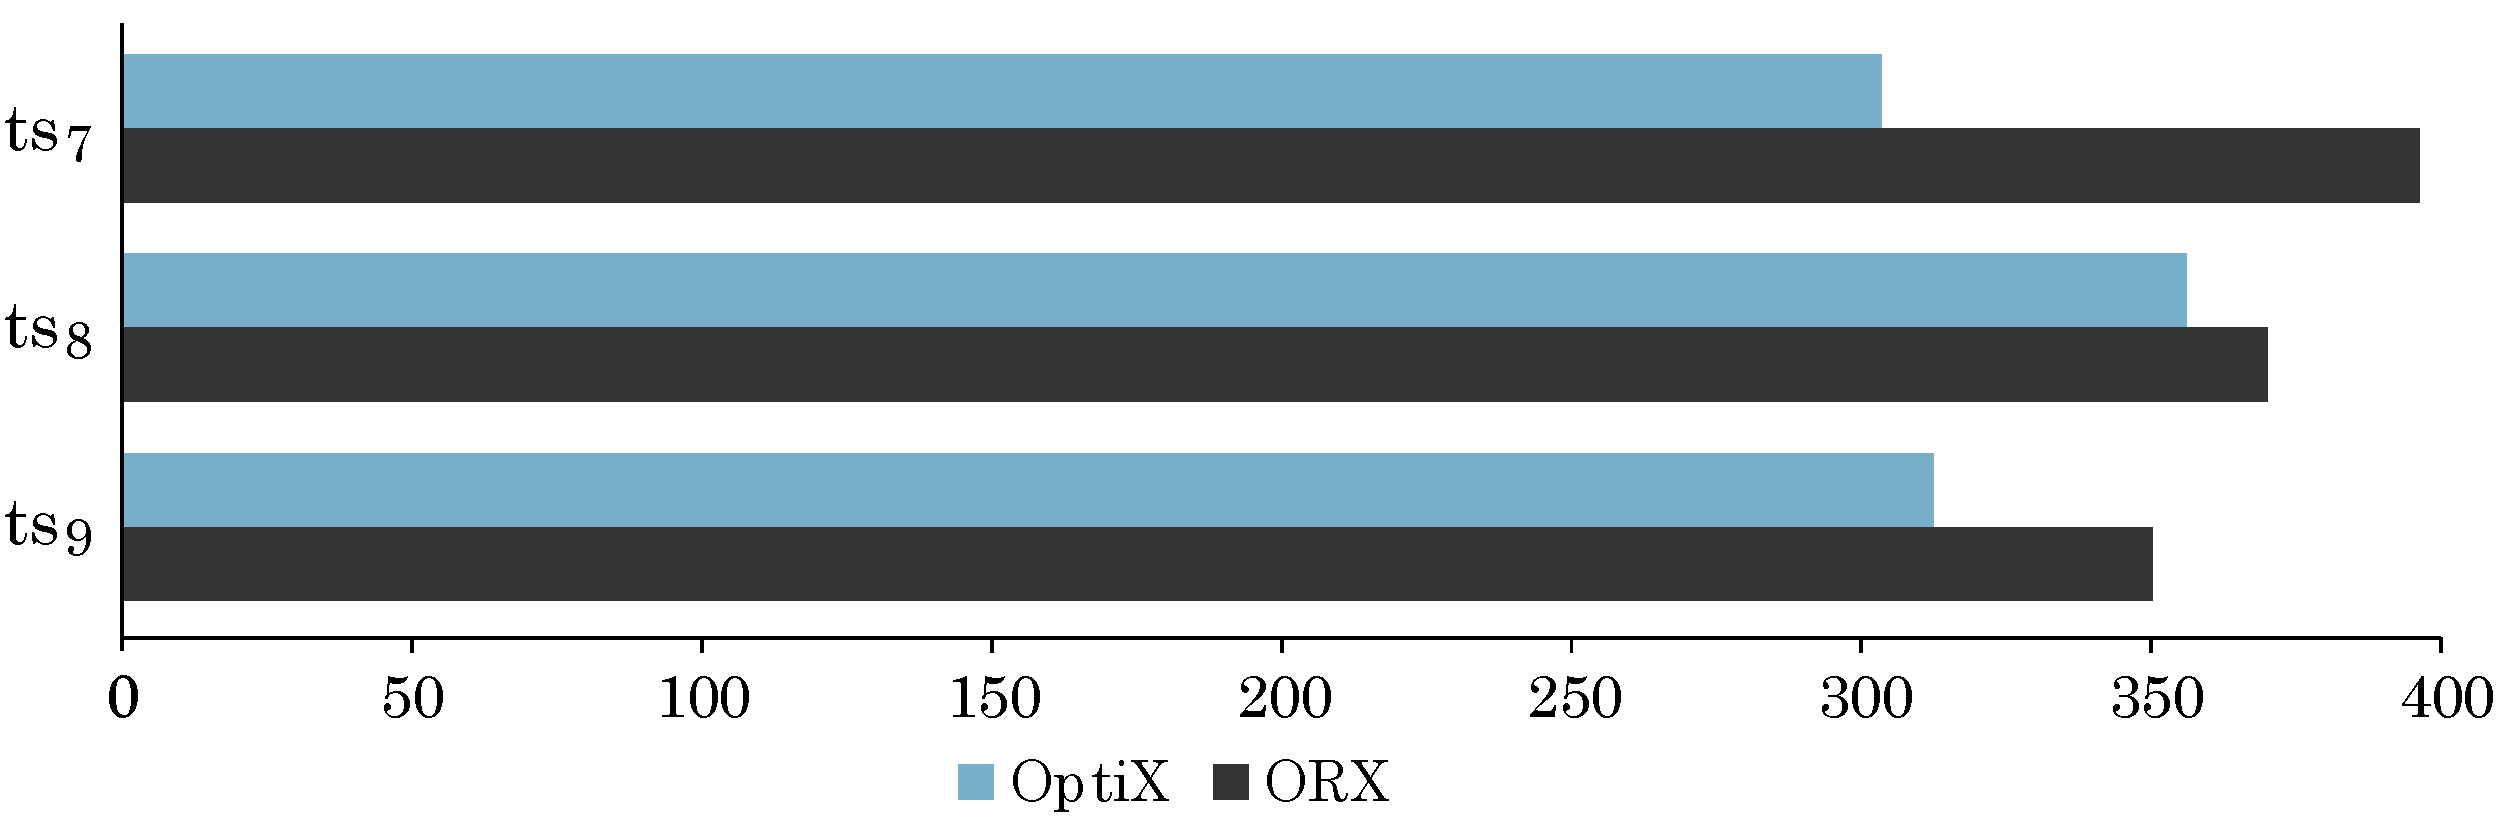
\includegraphics[width=\textwidth]{figures/test_results/3.pdf}
    \caption{Results from Test Data Collection 3 in Experimental Evaluation}
    \label{3rd_test_set}
\end{figure}

The third collection of test sets consisted of $ts_7$, $ts_8$ and $ts_9$, with 200 tests and 50 test machines, and was designed to test the mechanisms in situations with more realistically number of tests, and a fair number of machines.

Figure \ref{3rd_test_set} shows that OptiX once again provided better total results for all of the test sets in the collection. OptiX finished searching after 1.72, 0.22 and 0.67 seconds respectively for the three test sets, while ORX again was timed out after 30 seconds.

$ts_7$, which was the test set with the largest number of possible solutions, was also the one where the difference between the two mechanisms were the most distinct as the total difference was 92.67 seconds. The two remaining differences were not as conspicuous. An interesting trait that was discovered was that ORX provided a 17 second shorter execution time for $ts_8$ than OptiX accomplished. However, by using 30 seconds to find this solution, OptiX still provided a better total time. This demonstrates that it is not enough to find an allocation in which the execution time is minimized; it is also important to minimize the time taken to find the solution. 

\begin{figure}[t]
    \centering
    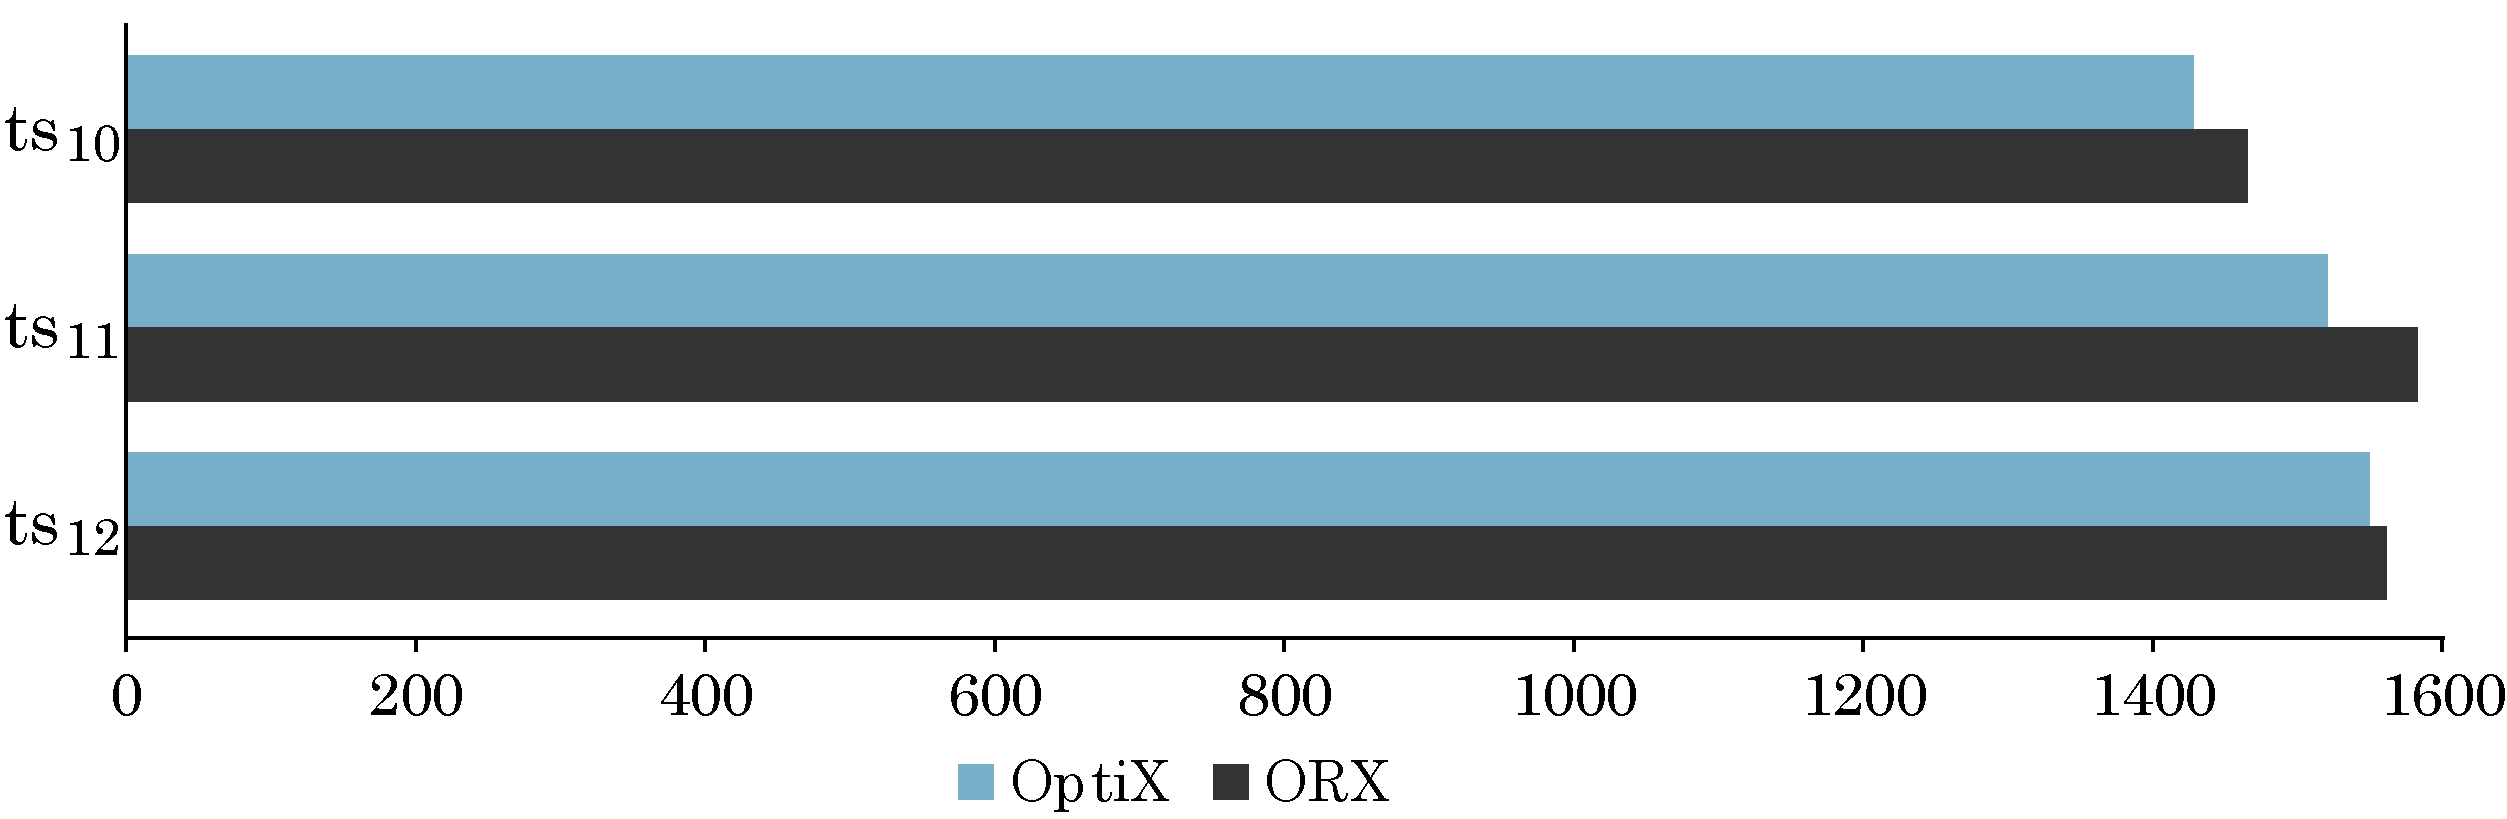
\includegraphics[width=\textwidth]{figures/test_results/4.pdf}
    \caption{Results from Test Data Collection 4 in Experimental Evaluation}
    \label{4th_test_set}
\end{figure}

The fourth and last collection of test sets consisted of $ts_{10}$, $ts_{11}$ and $ts_{12}$, with 200 tests and 10 test machines, and was designed to test the mechanisms in situations with realistic numbers of both tests and machines in terms of the context the mechanism will be used in at Altibox.

Again, OptiX produced better results for all of the test sets, which can be seen in Figure \ref{4th_test_set}. As with collection 3, the differences in results were not as outstanding for this collection as for the two first ones. This is likely due to a much more limited amount of possible solutions to the problem, as the number of test machines was small and the number of tests moderate.

The largest difference in execution time was a mere 33 seconds for $ts_{11}$. Again, ORX produced a better solution of execution time for $ts_{12}$, but since OptiX used less than a second to find its solution for this and the remaining test sets, and ORX again was timed out after 30 seconds for the whole collection, OptiX provided the overall best result of 1549.80 seconds, which was 11.26 seconds less than the total time found by ORX for this problem.

%\begin{center}* * *\end{center}
\begin{center}------------------------------\end{center}

\noindent OptiX provided better results than ORX on all of the test sets in the collection. The searching time was generally exceptional, aside from for $ts_1$, where the searching was timed out after 30 seconds, and $ts_2$, where the searching time was more than 8 seconds. Compared to the searching times of ORX, OptiX did a better job on every test set.

It is a clear trend that ORX requires a lot of time to find good results, and that the quality of the final results most of the time is poor compared those of OptiX. Both mechanisms were timed out upon solving the problem with the largest amount of combinatorial solutions, but the total time of ORX' result was nevertheless 147\% of that of OptiX'.

However, ORX found better execution times for $ts_8$ and $ts_12$, which means that even though OptiX provided better overall results, the mechanism still has potential for improvement. Although OptiX performed better that the benchmark values for all test sets, the difference between the results provided by the two mechanisms was generally not tremendous. This was especially the case for collection 4, which is the most realistic scenario covered by the experimental evaluation.

OR-tools is an excellent library for solving CP and combinatorial problems, but OptiX provided better results in this specific problem. A contributing factor to can be explained by OptiX being designed and implemented specifically to solve this type of problem efficiently, whereas OR-tools was designed to provide feasible solutions to a much broader range of problems. It is therefore not guaranteed to make the best decisions at any point of the process, so the time taken to identify good solutions is inclined to take more time. This is likely the reason why ORX did not stop before the timeout of 30 seconds on any of the test sets, whereas OptiX used less than a second on most of them.

\subsection{Threats to Validity}

Judging from the results obtained in the previous section, it is clear that OptiX is performs superior compared to ORX in the experiments. It is therefore important to establish some possible contributing factors that may threaten the validity of the results.

As explained in the previous section, the test data was randomly generated. This means that there might have been some degree of chance involved, and that if the test sets were generated again, other results may be obtained. Additionally, there might have been some interesting situations in which to test the performance of the allocation mechanisms, that are not covered in the experimental evaluation. Even though the author tried their best to come up with realistic and representative scenarios to cover the allocation mechanism in full measure, there might have been some relevant scenarios that were not tested. Also, there might be some scenarios that would provide value despite being deemed pointless to test by the author.

The results may also depend on the performance of the machine that the experiments were conducted on. Had the experiments been conducted on a newer and faster machine with more available resources or a different operating system, the results would likely come out slightly different. ORX would perhaps be able to reach better solutions before being timed out, and could thus possibly be a stronger competitor, whereas the results obtained by OptiX would not likely be affected as much, as most of the problems were solved in less than a second.

Another contributing factor may be the author's knowledge of and experience with OR-tools being far from optimal. With limited documentation and general online and literary coverage, exploring every corner of the library just could not be done with a narrow time-frame and other tasks that had to be prioritized. Although the author did invest a fair amount of time and energy in getting acquainted with the tools and tried their best to implement ORX to be as strong of a competitor to OptiX as possible, it may be a very real possibility that there are ways to implement it that would provide greater efficiency. Another possibility is that there are other optimization libraries that could potentially accomplish better results in this optimization problem than OR-tools.

\subsection{Discussion}
\improvement[inline]{TODO}
\comment{Selenium and Selenium Grid.

Noe om objektivet at prosjektet.

It is not necessary to be a highly skilled programmer to write Selenium test scripts, although some technical knowledge is required.


Egner seg spesielt godt til å kjøre store testsett og optimalisere kjøretiden

}












\subsection{Return on Investment}

Altibox has great interest in how incorporating \toolname \space to their testing process can affect their company from a business perspective. This section aims to enlighten some of these aspects.

All of the frameworks used in the development of \toolname \space are open-source. It has therefore not been necessary to pay for any licenses. \toolname \space itself is also handed to Altibox with no charges, so the associated investment solely consists of time and resources.

A priority during the design phase has been to create a user-friendly, intuitive and consistent interface. Building the website on the Django framework has rendered this an easy task. Getting to know the interface and learning to use it is thus not expected to be require excessive amounts of time and effort. Also, a brief user manual is included both on the website and in the appendix of this thesis.

As with test automation in general, writing test scripts for \toolname \space requires some technical knowledge. Being acquainted with the Python programming language and the Selenium library is a necessity. Writing these scripts will also take time, and additional time associated with maintaining said scripts should be expected. Furthermore, at least one computer, preferably more, should be available solely to be used for \toolname.

The success of applying \toolname \space partially depends on how the product is used. As explained in Chapter \ref{chapter.background}, caution should be used upon determining the automation coverage and which exact test that should be automated. The media content in TV Overalt is dynamic, as new movies and TV shows are released and made available, while old content is removed after a while. Thus, content-based tests are not likely to be durable, and will presumably require regular maintenance. Attempting to automate everything is also an approach that is almost guaranteed to fail \cite{ksljdf}.

But there are a lot of benefits to \toolname \space too, if used correctly. One of these benefits is significantly extended test coverage. Currently, TV Overalt is available in Chrome, Edge, Firefox, Internet Explorer and Safari. During an acceptance test, the test team often has limited amount of time, which means that they will not be able to perform all of the tests in all browsers, and have to select which browsers should be tested. This will most likely no longer be a problem after incorporating \toolname, as each test script can be executed in all of these browsers. Once the test scripts are written and in working order, they can be executed rapidly, precisely and repeatedly with no additional expenses and virtually no time used by human resources, and in \improvement{Except Safari?} all of the aforementioned browsers with only a few keystrokes. The remaining time can thus be used for manually conducting the tests unsuited for automation. This way, it will now be possible to cover all of the supported browsers even with a limited time frame, and thus be able to test the test object more thoroughly and detect more defects.

Detecting more defects will likely result in improved product quality, and by extension additional time to test the product to an even greater extent. Other effects of this could be fewer customer inquiries and higher customer satisfactory, which could lead to increased customer confidence in the product as well as in the company.

Another strength to \toolname \space is that even though developing test scripts is a task that requires technical staff, once the scripts are written and uploaded, no technical background is needed to execute the tests, which would be the case without the user interface of \toolname.

As explained in the previous section, writing Selenium tests generally does not require advanced programming skills and is not immensely time-consuming. The code involved is fairly simple, as it is mostly compromised of locating web elements based on the class or id names, or similar, of the elements in the HTML code, and clicking buttons or filling out text fields. The time used for test script coding and maintenance will likely take approximately the same amount of time as a few manual executions of the same test, and thus provide great value in the long term.

As opposed to some other cloud testing services which execute tests on remote machines in distant locations, \toolname \space can execute tests on un-deployed versions of the test object, that are only available on the network that the \toolname \space server is connected to. In practice, this means that the tests uploaded to \toolname \space can be executed on the test object before it is deployed, and thus be able to identify defects earlier.

\toolname \space provides a JIRA integration that will enable the testers to save a lot of time on reporting failed test executions to the issue tracking system, which will be of great value. Locating issues linked to a specific test can also be done without having to open the JIRA website and search for issues with specific attribute values that comply with the specific test.










\comment{- What is needed in order for the product to be used (Learning to set up and use the tool, dedicated machines, learning to write automated tests and learning to use optiruns template for automated tests, learning python if they don't know it already)
- Was it worth it (for Altibox)?
- How optirun competes with alternative tools
- Compare to current test process?


This chapter will include:\\
- Research questions\\
- Thorough performance comparison of optx and orx - use graphs!\\
- Evaluation of allocation mechanism\\
- Discussion of complete system\\
- Discussion of how \toolname \space can affect Altibox' overall testing process of TV Overalt (time saved or more time used to write tests? Human mistakes avoided if tests are written well, etc.). Compare to how the test process has previously been.


The existing test process will be discussed in Chapter \ref(chapter.discussion).
Test automation has previously been completely omitted, and Altibox was avid to include this in the testing of their software products.
}

